\documentclass{article}
\usepackage{amsmath, amssymb, amsthm, url, hyperref}
\usepackage[T1]{fontenc}
\usepackage[utf8]{inputenc}
\usepackage{cleveref}
\usepackage[thinc]{esdiff}
\usepackage{commath}
\usepackage{pgfplots}
\usepackage{enumitem}

\newtheorem{theorem}{Theorem}

\begin{document}
	\begin{theorem}{(Potters Theorem)}
		\begin{enumerate}[label=(\roman*)]
			\item If $l$ is slowly varying function then for any chosen constants $A>1$, $\delta>0$ there exits $X=X(A, \delta)$ such that
			\[
			\frac{l(y)}{l(x)}\le A\max\left\{\left(\frac{y}{x}\right)^{\delta}, \left(\frac{x}{y}\right)^{\delta}\right\} \quad (x\ge X, y\ge X)
			\]
			
			\item If further, $l$ is bounded away from $0$ and $\infty$ in every compact subset of $[0, \infty)$, then for every $\delta>0$ there exists $A'=A'(\delta)>1$ such that
			\[
			\frac{l(y)}{l(x)}\le A'\max\left\{\left(\frac{y}{x}\right)^{\delta}, \left(\frac{x}{y}\right)^{\delta}\right\} \quad (x\ge 0, y\ge 0)
			\]
			
			\item If $f$ is regularly varying of index $\rho$ then for any chosen $A>1$, $\delta>0$ there exists $X=X(A, \delta)$ such that 
			\[
			\frac{f(y)}{f(x)}\le A\max\left\{\left(\frac{y}{x}\right)^{\rho+\delta}, \left(\frac{x}{y}\right)^{\rho+\delta}\right\} \quad (x\ge 0, y\ge 0)
			\]
		\end{enumerate}
	\end{theorem}
	
	\begin{figure}
		\centering
		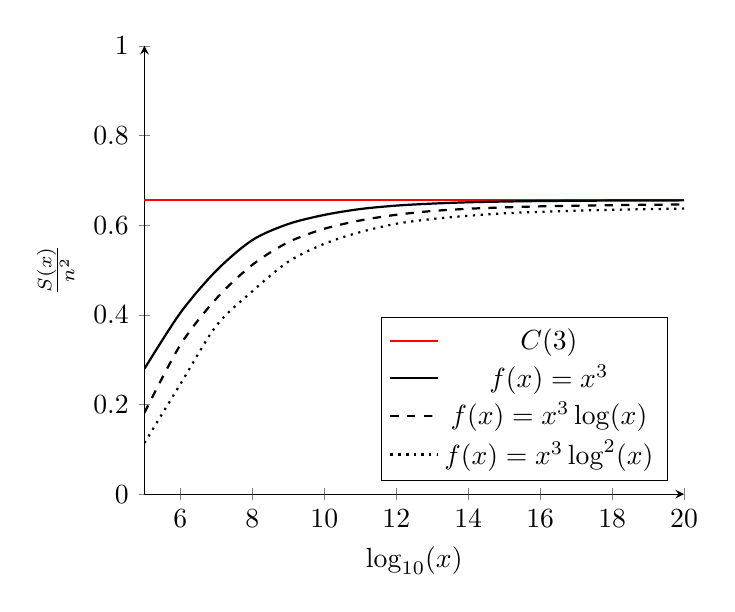
\begin{tikzpicture}
			\begin{axis}
				[
					ymode=normal,
					axis lines=left,
					xlabel=$\log_{10}(x)$,
					ylabel=$\frac{S(x)}{n^2}$,
					ymin=0,
					ymax=1,
					legend pos=south east,
				]
				\addplot[red, thick, domain=5:20] {0.655514388573};
				\addlegendentry{$C(3)$}
				\addplot[smooth, thick] table{
					5 	 0.279586
					6 	 0.404537
					7 	 0.498704
					8 	 0.566753
					9 	 0.602608
					10	 0.622818
					11	 0.63592
					12	 0.643569
					13	 0.648045
					14	 0.65099
					15	 0.652635
					16	 0.653749
					17	 0.654374
					18	 0.654807
					19 	 0.655054
					20	 0.655219
				};
				\addlegendentry{$f(x)=x^3$}
				\addplot[smooth, dashed, thick] table{
					5 0.181406
					6 0.333045
					7 0.436385
					8 0.51158
					9 0.562007
					10 0.591895
					11 0.610496
					12 0.623089
					13 0.631517
					14 0.636507
					15 0.639613
					16 0.641916
					17 0.643398
					18 0.64458
					19 0.645429
					20 0.64612
				};
				\addlegendentry{$f(x)=x^3\log(x)$}
				\addplot[smooth, dotted, thick] table{
					5 0.114187
					6 0.245542
					7 0.375879
					8 0.452546
					9 0.518537
					10 0.558425
					11 0.584521
					12 0.603029
					13 0.613707
					14 0.620829
					15 0.626311
					16 0.629712
					17 0.632283
					18 0.634184
					19 0.635672
					20 0.636922	
				};
				\addlegendentry{$f(x)=x^3\log^2(x)$}
			\end{axis}
			
		\end{tikzpicture}
		\caption{Example on how the slowly varying part affects convergence}
		\label{SVeffectsOnConvergence}
	\end{figure}
	
	\begin{figure}
		\centering
		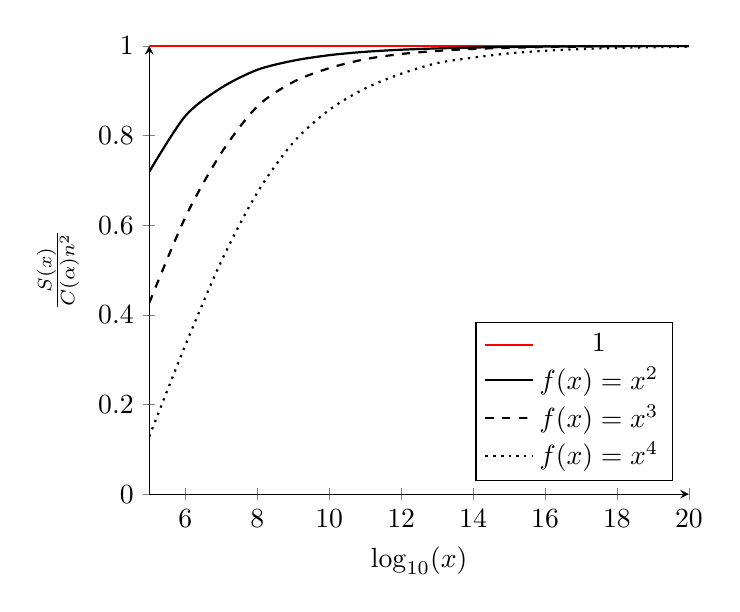
\begin{tikzpicture}
			\begin{axis}
				[
					ymode=normal,
					axis lines=left,
					xlabel=$\log_{10}(x)$,
					ylabel=$\frac{S(x)}{C(\alpha)n^2}$,
					ymin=0,
					ymax=1,
					legend pos=south east,
				]
				\addplot[red, thick, domain=5:20] {1};
				\addlegendentry{$1$}
				\addplot[smooth, thick] table{
					5 0.7190649474
					6 0.8432680421
					7 0.9062543204
					8 0.9463711807
					9 0.9668099942
					10 0.9791124528
					11 0.9866137034
					12 0.991276796
					13 0.9942134461
					14 0.9961380048
					15 0.997401421
					16 0.9982504911
					17 0.9988154056
					18 0.999195789
					19 0.9994539063
					20 0.9996293808
				};
				\addlegendentry{$f(x)=x^2$}
				\addplot[smooth, dashed, thick] table{
					5 0.4265139025
					6 0.6171290929
					7 0.7607826902
					8 0.8645927685
					9 0.9192902711
					10 0.9501210208
					11 0.9701083776
					12 0.9817770765
					13 0.9886053019
					14 0.9930979569
					15 0.9956074365
					16 0.9973068653
					17 0.998260315
					18 0.9989208649
					19 0.9992976682
					20 0.999549379
				};
				\addlegendentry{$f(x)=x^3$}
				\addplot[smooth, dotted, thick] table{
					5 0.1286654854
					6 0.3315713285
					7 0.5190241531
					8 0.6722635208
					9 0.7841729099
					10 0.8569712311
					11 0.9049426154
					12 0.9377017748
					13 0.9614184049
					14 0.9736709469
					15 0.9830932284
					16 0.9889955649
					17 0.9928220363
					18 0.99533385
					19 0.9968852143
					20 0.9980551234
				};
				\addlegendentry{$f(x)=x^4$}
			\end{axis}
			
		\end{tikzpicture}
		\caption{Example on how the index affects convergence}
		\label{indexEffectsOnConvergence}
	\end{figure}
\end{document}